\chapter{Implementacija i korisničko sučelje}
		
		
		\section{Korištene tehnologije i alati}
		

			

			 \textit{}Za komunikaciju u timu koristila se aplikacija WhatsApp\textsuperscript{1} i Discord\textsuperscript{2}. Glavni sustav za upravljanje kodom bio je Git\textsuperscript{3}, dok se udaljeni direktorij projekta nalazi se na web platformi GitHub\textsuperscript{4}. Za izradu UML dijagrama korišten je alat Astah UML\textsuperscript{5}. Kao integrirano razvojno okruženje koristili smo Microsoft Visual Studio\textsuperscript{6}. Namijenjen je ponajviše za razvoj računalnih softvera napisanih u C, C++, C#, Java Script i drugih. Pruža dosljedno iskustvo na Windowsima, macOS-u i Linuxu.
			 
			 U aplikaciji je za backend korišten radni okvir Flask\textsuperscript{7} i jezik Python\textsuperscript{8}, a za frontend React\textsuperscript{9} i jezik JavaScript\textsuperscript{10}. Frontend u Reactu je bio predožen od strane mentora dok smo backend odabrali sami raditi u pythonu. React, još poznat kao React.js ili ReactJS, je biblioteka u JavaScriptu za izgradnju korisničkih sučelja. Održava ju Facebooka. Njegova arhitektura se temelji na komponentama. Komponente predstavljaju klase ili funkcije koje prihvaćaju unos i na temelju unosa prikazuju različite HTML elemente.
			 
			 \footnotetext[1]{\url{https://www.whatsapp.com/}}
			 \footnotetext[2]{\url{https://discord.com/}}
			 \footnotetext[3]{\url{https://git-scm.com/}}
			 \footnotetext[4]{\url{https://github.com/}}
			 \footnotetext[5]{\url{https://astah.net/products/astah-uml/}}
			 \footnotetext[6]{\url{https://visualstudio.microsoft.com/}}
			 \footnotetext[7]{\url{https://flask.palletsprojects.com/en/3.0.x/}}
			 \footnotetext[8]{\url{https://www.python.org/}}
			 \footnotetext[9]{\url{https://reactjs.org/}}
			 \footnotetext[10]{\url{https://www.javascript.com/}}
			 
			
			\eject 
		
	
		\section{Ispitivanje programskog rješenja}
			
			
			\subsection{Ispitivanje sustava}
			
			 \textit{} Ispitivanje sustava ostvareno je pomoću Selenium IDE snimanjem korisnikovih akcija radi automatskog ponavljanja ispita
			 \begin{itemize}
			 	\item Prvi slučaj - ulaz
			 			\begin{enumerate}
			 				\item Otvaranje početne stranice u web pregledniku
			 				\item Registracija s postojećom mail adresom
			 				\item Login s nepotpunom e-mail adresom (izostavljamo znak @), lozinkom i bez reCAPTCHA-e
			 				\item Login s pogrešnom lozinkom i bez reCAPTCHA-e
			 				\item Login s pogrešnom lozinkom
			 				\item Login s točnim podacima
			 				\item Logout
			 			\end{enumerate}
			 	\item Prvi slučaj - očekivani rezultati
			 			\begin{enumerate}
			 				\item Prikazuje se početna stranica koja nudi registraciju i login
			 				\item Javlja se greška "Račun s ovim emailom već postoji."
			 				\item Pojavljuje se napomena "Uključite znak @ u e-adresu."
			 				\item Javlja se greška "Molimo da riješite reCAPTCHA-u prije nastavka"
			 				\item Javlja se greška "Pogrešan e-mail ili lozinka"
			 				\item Korisnik se prijavljuje te se otvara stranica s konferencijama
			 				\item Korisnik se odjavljuje te se otvara stranica za login
			 			\end{enumerate}
			 	\item Prikaz rezultata
			 			\begin{figure}[htb]
			 				\centering
			 				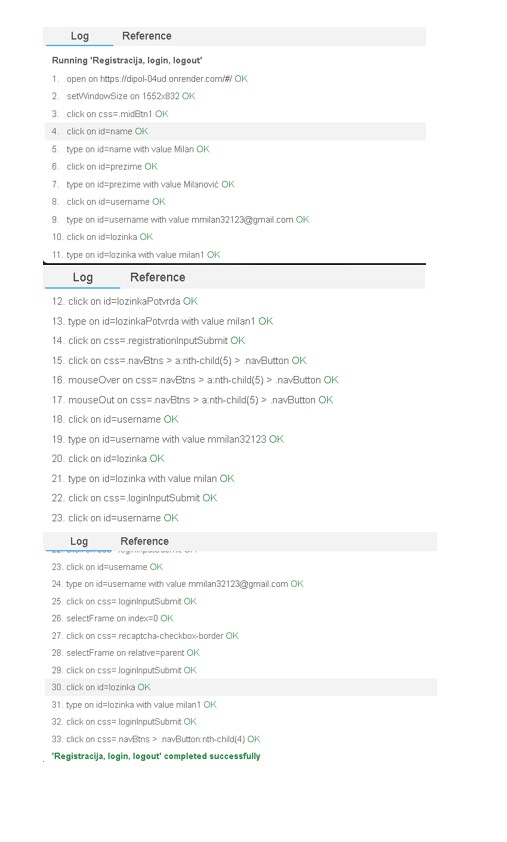
\includegraphics[width=8cm]{slike/test_1.jpg}
			 				\caption{test 1}
			 				\label{fig:fer-logo}
			 			\end{figure}
			 \end{itemize}
			 
			 \newpage
			 
			 \begin{itemize}
			 	\item Drugi slučaj - ulaz
			 	\begin{enumerate}
			 		\item Otvaranje stranice s konferencijama u web pregledniku
			 		\item Pritisćemo tipku "Pristupi" na nekoj od konferencija
			 		\item Unosimo pogrešnu lozinku za konferenciju
			 		\item Unosimo ispravnu lozinku za konferenciju
			 		\item Pritišćemo tipku "VOTE" za neki radi
			 		\item Pritišćemo tipku "VOTE" za neki drugi rad
			 	\end{enumerate}
			 	\item Drugi slučaj - očekivani rezultati
			 	\begin{enumerate}
			 		\item Prikazuju se sve aktivne i nadolazeće konferencije te vremenska prognoza za aktivne konferencije
			 		\item Prikazuje nam se polje za upis lozinke za konferenciju
			 		\item Iskače skočni prozor koji nam govori da lozinka nije ispravna
			 		\item Ulazimo u konferenciju gdje nam se prikazuju radovi
			 		\item Glasamo za taj rad, te sada na tipci piše "VOTED"
			 		\item Ništa se ne dogodi jer nam nije dopušteno glasati za više od jednog rada
			 	\end{enumerate}
			 	\item Prikaz rezultata
			 	\begin{figure}[htb]
			 		\centering
			 		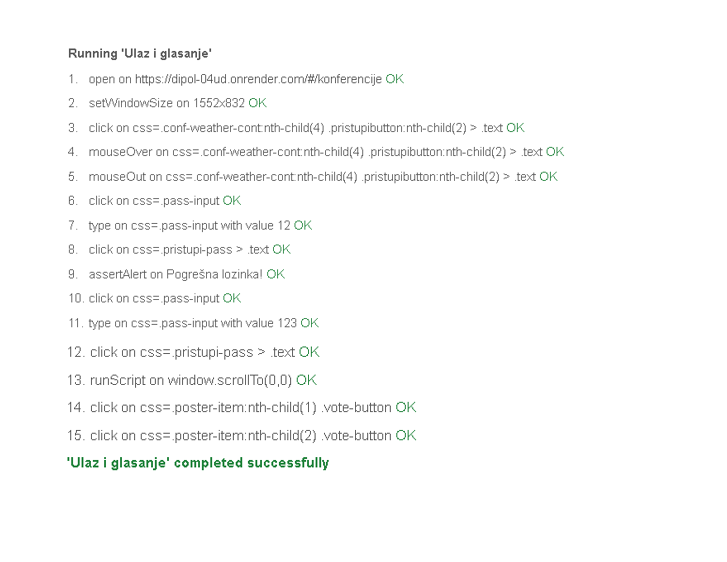
\includegraphics[width=11cm]{slike/test_2.png}
			 		\caption{test 2}
			 		\label{fig:fer-logo}
			 	\end{figure}
			 \end{itemize}
			 
			 \newpage
			 
			 \begin{itemize}
			 	\item Treći slučaj - ulaz
			 	\begin{enumerate}
			 		\item Otvaranje stranice za prošle konferencije u web pregledniku
			 		\item Pritinemo tipku "Pregledaj rezultate"
			 		\item Pritinemo tipku "Galerija fotografija"
			 		\item Pritisnemo svaku fotografiju jednom
			 		\item Pritisnemo tipku "Preuzmi odabrane fotografije"
			 	\end{enumerate}
			 	\item Treći slučaj - očekivani rezultati
			 	\begin{enumerate}
			 		\item Prikazuju se sve prošle konferencije
			 		\item Otvara se stranica s rezultatime te konferencije
			 		\item Otvara se galerija sa svim slikama te konferencije
			 		\item Svaka fotografije se označuje (obrub mijenja boju)
			 		\item Svaka se fotografije preuzima lokalno na uređaj
			 	\end{enumerate}
			 	\item Prikaz rezultata
			 	\begin{figure}[htb]
			 		\centering
			 		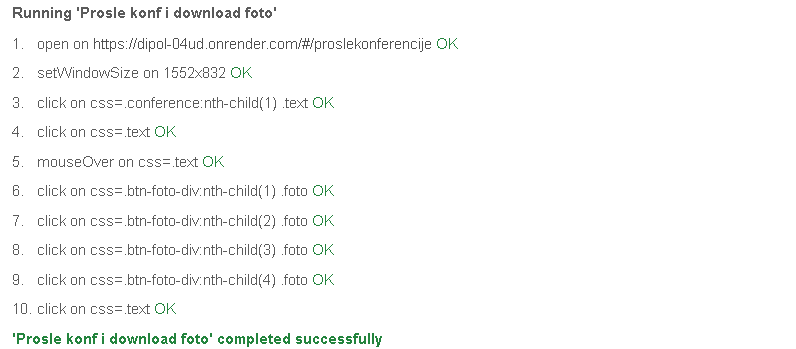
\includegraphics[width=11cm]{slike/test_3.png}
			 		\caption{test 3}
			 		\label{fig:fer-logo}
			 	\end{figure}
			 \end{itemize}
			 
			 \newpage
			 
			 \begin{itemize}
			 	\item Četvrti slučaj - ulaz
			 	\begin{enumerate}
			 		\item Otvaranje stranice s konferencijama u web pregledniku
			 		\item Pritisnemo tipku "Dodaj konferenciju"
			 		\item Pritisnemo tipku "Unesi" bez da unesemo sve podatke
			 		\item Pritisnemo tipku "Unesi" nakon što smo unijeli sve podatke, ali nismo u potpunosti unijeli datum ili vrijeme
			 		\item Pritisnemo tipku "Unesi" nakon što smo unijeli sve podatke, svi podaci su točni i potpuni
			 	\end{enumerate}
			 	\item Četvrti slučaj - očekivani rezultati
			 	\begin{enumerate}
			 		\item Prikazuju se sve aktivne i nadolazeće konferencije te vremenska prognoza za aktivne konferencije
			 		\item Otvara se stranica za dodavanje konferencije
			 		\item Pojavljuje se napomena da ispunimo prvo po redu polje koje nije ispunjeno
			 		\item Pojavljuje se napomena kod polja za datum ili vrijeme koja glasi "Unesite važeću vrijednost. Ovo je polje nepotpuno ili sadrži nevažeći datum."
			 		\item Vraćamo se na stranicu s konferencijama te ako smo unijeli datum koji je već prošao, konferencija se prikazuje na stranici "Prošle konferencije"
			 		\item Vraćamo se na stranicu s konferencijama te ako smo unijeli tek nadolazeći datum, konferencija se prikazuje na stranici "Konferencije" pod "Nadolazeće konferencije"
			 		\item Vraćamo se na stranicu s konferencijama te ako smo unijeli datum početka prije trenutnog vremena, a datum završetka nakon trenutnog vremena, konferencija se prikazuje na stranici "Konferencije" pod "Aktivne konferencije"
			 	\end{enumerate}
			 	\item Prikaz rezultata
			 	\begin{figure}[htb]
			 		\centering
			 		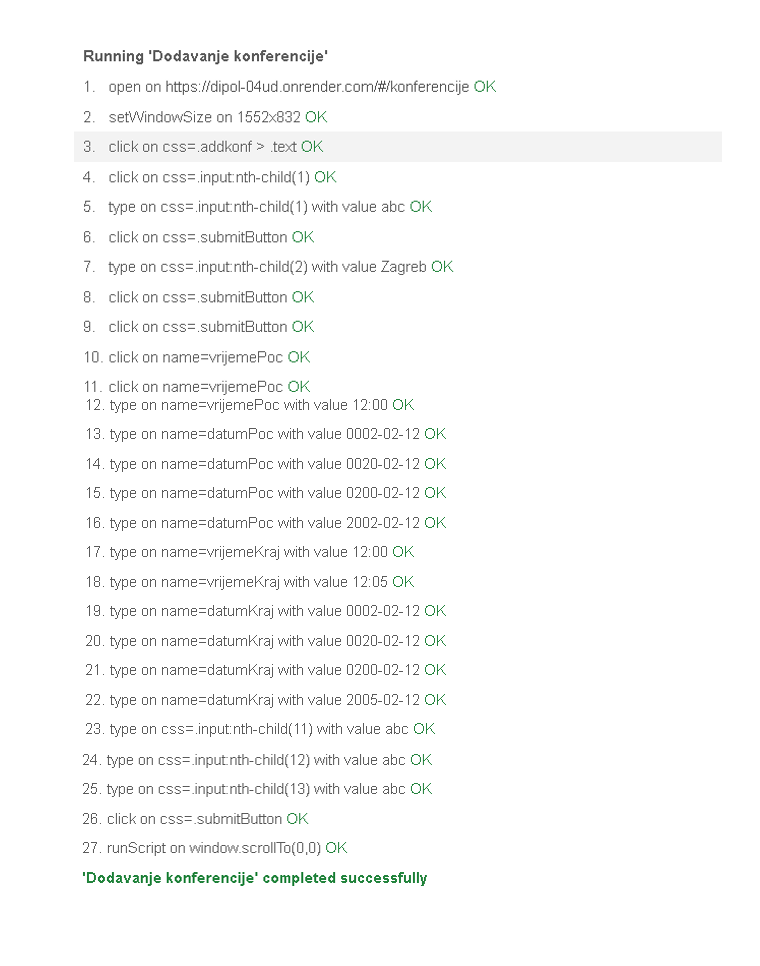
\includegraphics[width=11cm]{slike/test_4.png}
			 		\caption{test 4}
			 		\label{fig:fer-logo}
			 	\end{figure}
			 \end{itemize}
			 
			 \newpage
			 \newpage
			 
			 \begin{itemize}
			 	\item Peti slučaj - ulaz
			 	\begin{enumerate}
			 		\item Otvaranje stranice s konferencijama u web pregledniku
			 		\item Pod nadolazećim konferencijama pritisnemo tipku "Dodaj voditelja"
			 		\item Pritisnemo tipku "Unesi" bez da upišemo "Mail voditelja"
			 		\item Pritisnemo tipku "Unesi" s neispravno ispunjenim poljem "Mail voditelja"
			 		\item Pritisnemo tipku "Unesi" s ispravno ispunjenim poljem "Mail voditelja", ali ta e-mail adresa se ne nalazi u bazi podataka
			 		\item Pritisnemo tipku "Unesi" s ispravno ispunjenim poljem "Mail voditelja" i ta e-mail adresa se nalazi u bazi podataka
			 	\end{enumerate}
			 	\item Peti slučaj - očekivani rezultati
			 	\begin{enumerate}
			 		\item Prikazuju se sve aktivne i nadolazeće konferencije te vremenska prognoza za aktivne konferencije
			 		\item Otvara se stranica za dodavanje voditelja
			 		\item Pojavljuje se napomena "Ispunite ovo polje" (polje "Mail voditelja")
			 		\item Pojavljuje se napomena "Uključite znak @ u e-adresu."
			 		\item Javlja se greška "E-mail nije pronađen"
			 		\item Vraćamo se na stranicu s konferencijama
			 	\end{enumerate}
			 	\item Prikaz rezultata
			 	\begin{figure}[htb]
			 		\centering
			 		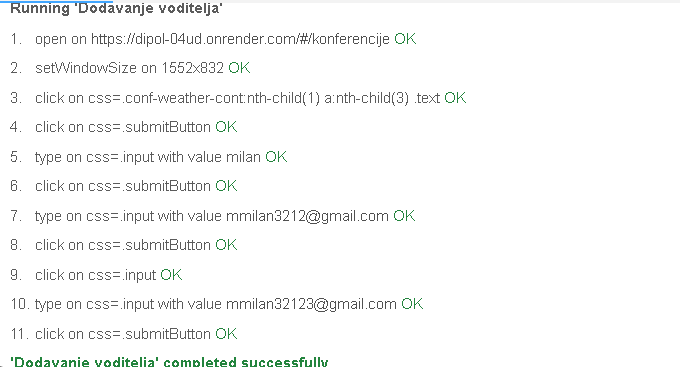
\includegraphics[width=11cm]{slike/test_5.png}
			 		\caption{test 5}
			 		\label{fig:fer-logo}
			 	\end{figure}
			 \end{itemize}
			 
			 	
			 	
			\eject 
		
		
		\section{Dijagram razmještaja}
			

			
			 \textit{}Dijagram razmještaja predstavlja strukturalni UML dijagram koji opisuje organizaciju sustava, fokusirajući se na međuodnos hardverskih i softverskih dijelova. Ključni elementi dijagrama uključuju čvorove, artefakte i poveznice. Čvorovi reprezentiraju stvarne uređaje (označeni stereotipom "device") ili izvođenja okoline (označena stereotipom "execution environment"), kao što su operativni sustav, virtualni strojevi na različitim razinama i slično. Artefakt predstavlja konkretnu realizaciju programske komponente, poput datoteka s izvornim ili izvršnim kodom, tablica u bazama podataka, skripti itd. Ovisnosti na dijagramu ilustriraju odnose među različitim artefaktima.
			 
			 Naš sustav temelji se na arhitekturi "klijent-poslužitelj", gdje se komunikacija između računala korisnika i računala poslužitelja odvija putem HTTP veze. Na računalu poslužitelja smješteni su web poslužitelj i poslužitelj baze podataka. Klijent, koristeći web preglednik, pristupa web aplikaciji.
			 
			 \begin{figure}[htb]
			 	\centering
			 	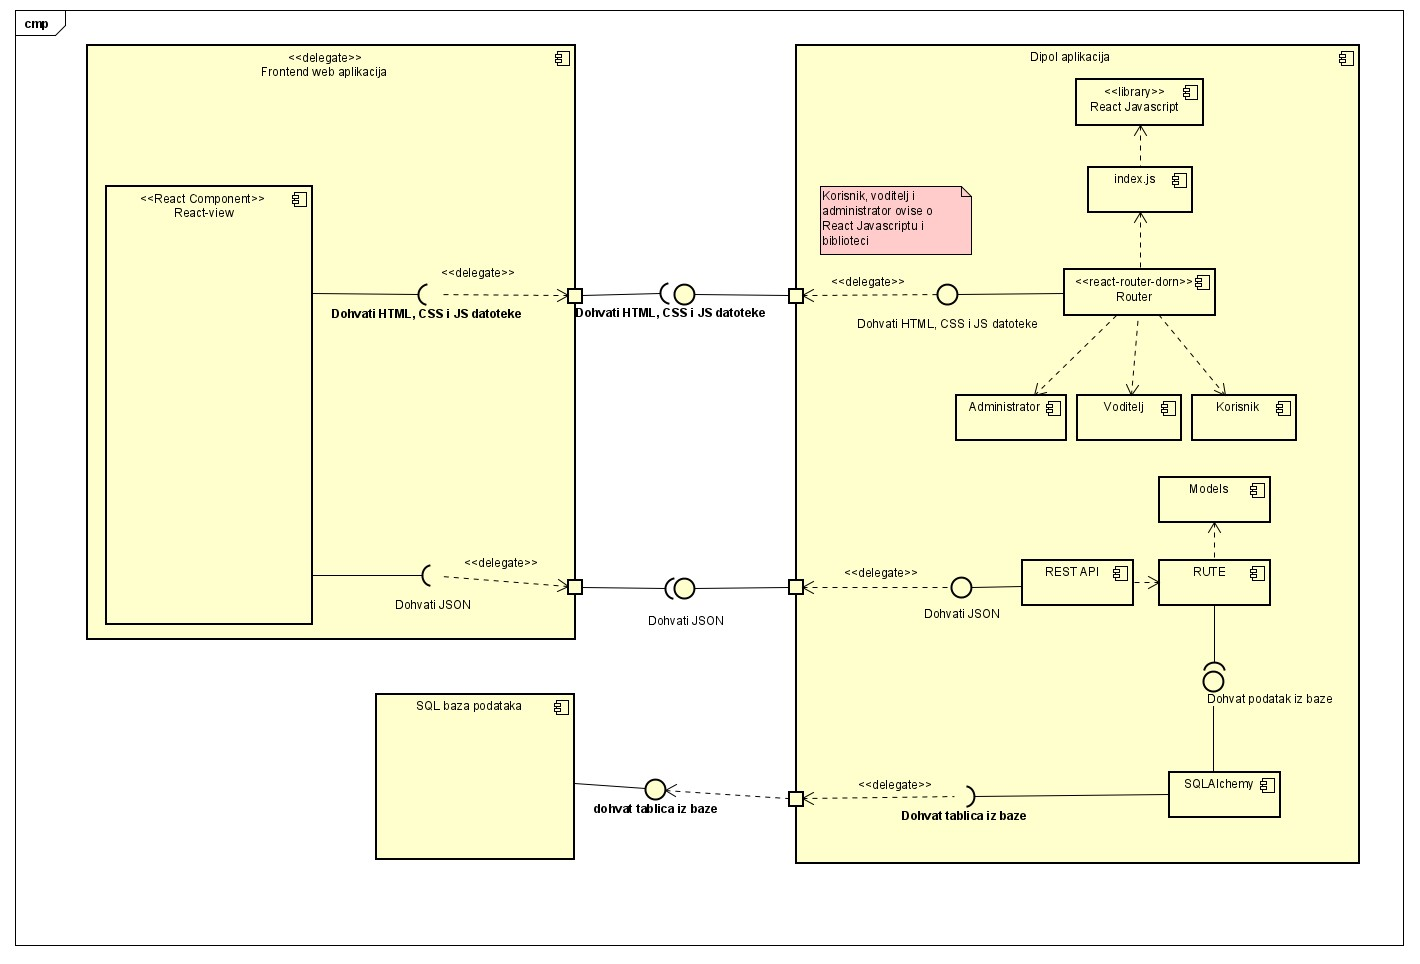
\includegraphics[width=11cm]{slike/Dijagram_komponensti.jpg}
			 	\caption{Dijagram razmještaja}
			 	\label{fig:fer-logo}
			 \end{figure}
			
			\eject 
		
		\section{Upute za puštanje u pogon}
		
			 \textit{}Aplikacija je puštena u pogon na javno dostupnom poslužitelju korištenjem besplatne usluge Render
			 
			 \subsection{Kreiranje baze podataka}
			 
			 	\text{} Baza podataka koju smo implementirali u aktivnoj verziji aplikacije je PostgreSQL, dok smo tijekom razvoja koristili pgAdmin bazu podataka. Na kontrolnoj ploči sustava Render, prilikom stvaranja nove baze podataka, odabiremo opciju PostgreSQL. Nakon toga, postavljamo naziv baze na "progi\textunderscore sri5", korisničko ime na "progi\textunderscore sri5\textunderscore user", dok je lozinka automatski generirana. Lokacija servera, odnosno regija gdje se baza podataka nalazi, je Frankfurt. Usluga nam omogućuje korištenje 1 GB besplatnog prostora za pohranu podataka.\\
			 	
			 	
				\begin{figure}[htb]
					\centering
					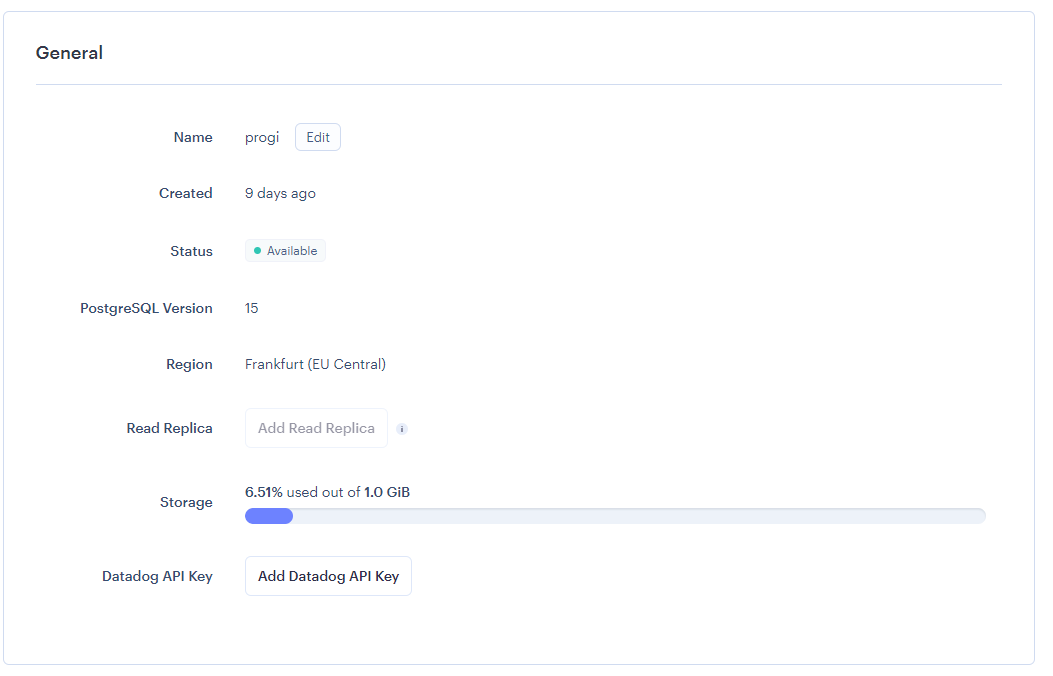
\includegraphics[width=15cm]{slike/baza_1.png}
					\caption{baza general}
					\label{fig:fer-logo}
				\end{figure}
				\newpage
				\begin{figure}[htb]
					\centering
					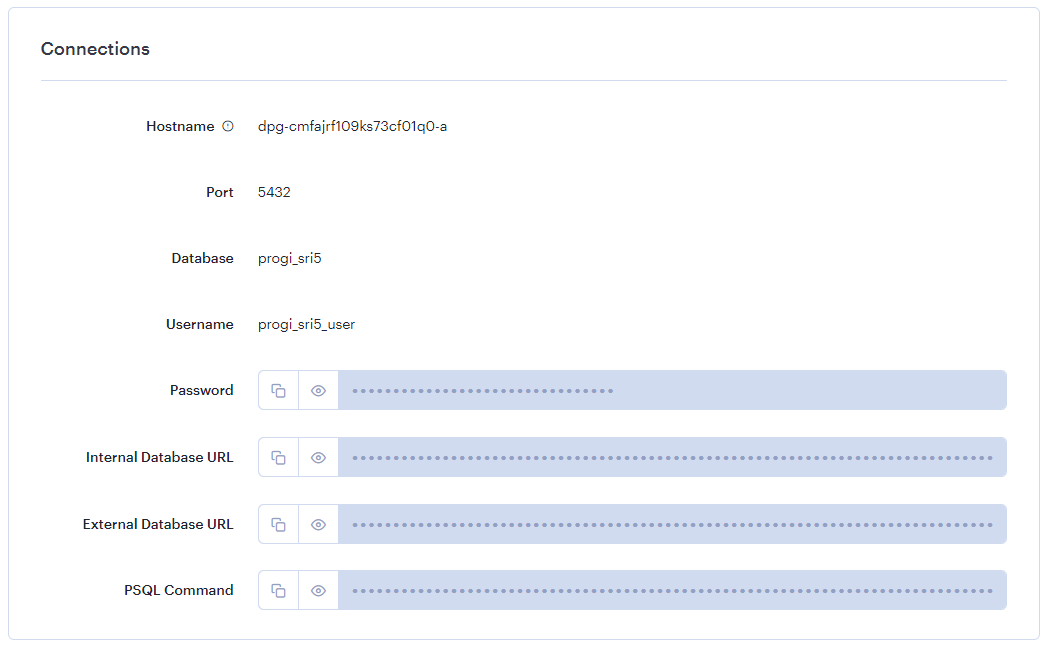
\includegraphics[width=15cm]{slike/baza_2.png}
					\caption{baza conection}
					\label{fig:fer-logo}
				\end{figure}
				
				\text{}Bazu podataka spajamo na pgAdmin V8 kako bi napravili potrebne tablice i atribute pomoću dobivenih podataka sa slike 5.8 te te podatke unosimo u prostor na slici 5.9 u pgAdmin nakon sto smo pritisnuli desni klin na "servers" -> "Register" -> "server".
				\newpage
				\begin{figure}[htb]
					\centering
					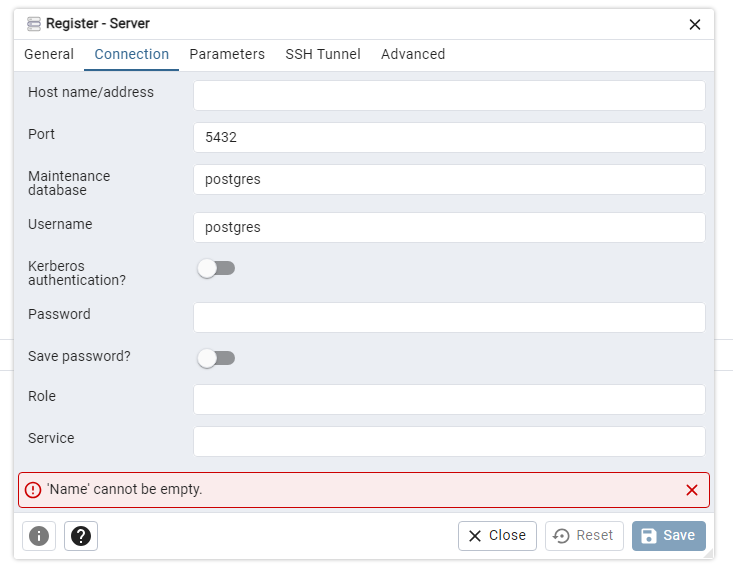
\includegraphics[width=15cm]{slike/server.png}
					\caption{Povezivanje baze na renderu}
					\label{fig:fer-logo}
				\end{figure}
				
			\subsection{Puštanje backend-a u pogon}
			
				\text{} Backend pustamo u pogon isto kao i bazu podataka na renderu. Pri pustanju Backenda u pogon na renderu prvo odabiremo gumb "New +" prikazan gore desno na priloženoj slici\\
			
			
				\begin{figure}[htb]
					\centering
					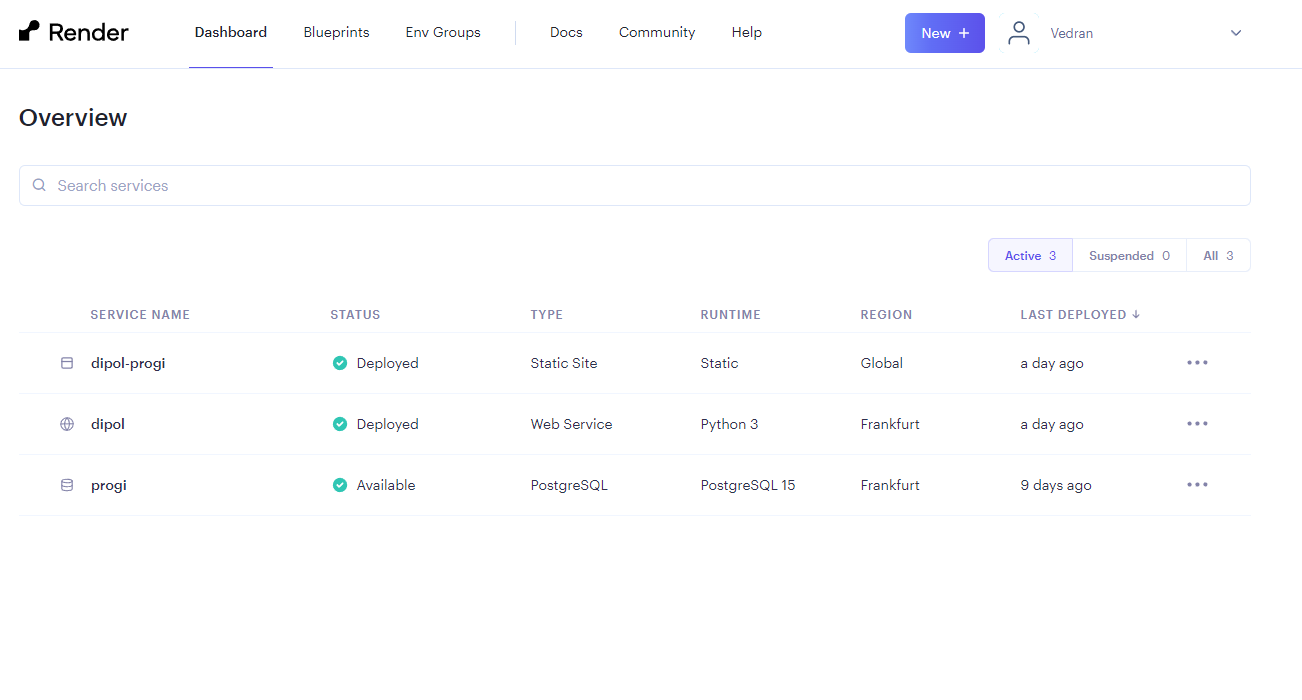
\includegraphics[width=15cm]{slike/back_1.png}
					\label{fig:fer-logo}
				\end{figure}
				\newpage
				\text{}Nakon toga odaibiremo opciju "Web service".\\
				
				\begin{figure}[htb]
					\centering
					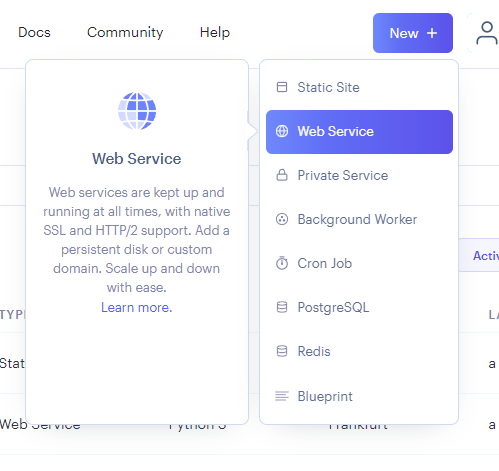
\includegraphics[width=10cm]{slike/back_2.png}
					\label{fig:fer-logo}
				\end{figure}
				\newpage
				\text{}Sada biramo kako je prikazanao na slici i pritišćemo gumb "Next".
				
				\begin{figure}[htb]
					\centering
					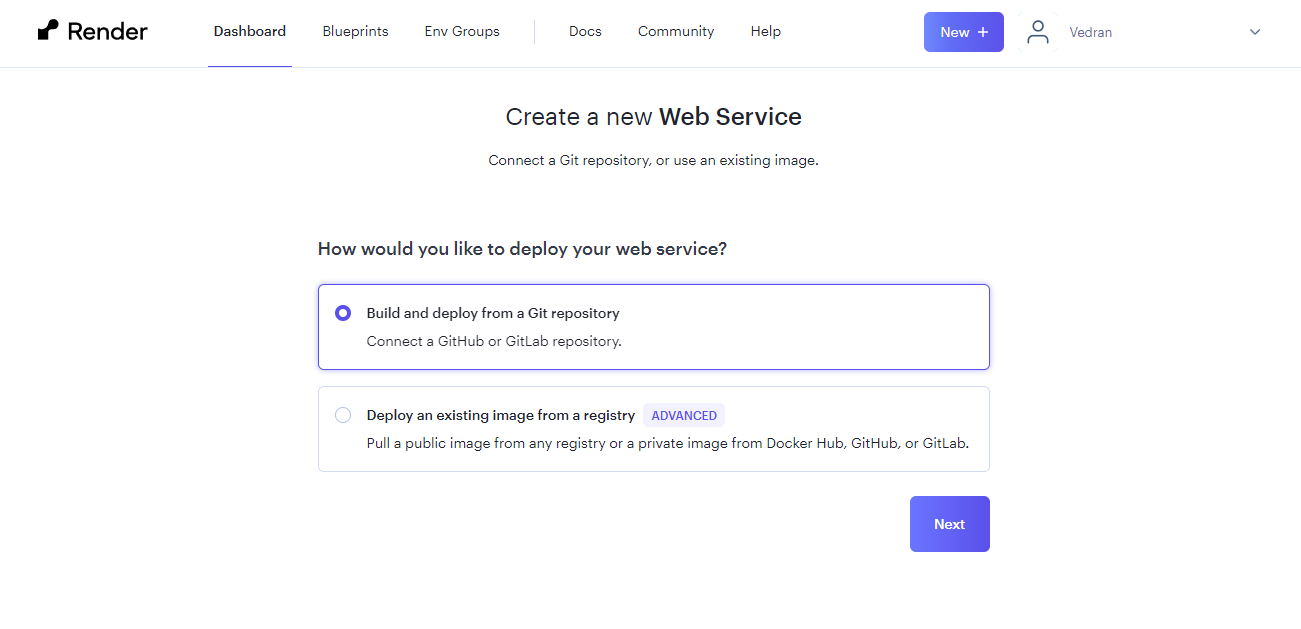
\includegraphics[width=15cm]{slike/back_3.png}
					\label{fig:fer-logo}
				\end{figure}
				\newpage
				\text{}Izabiremo server koji želimo pustiti u pogon te na stišćemo na njegov gumb "Connect".
				
				\begin{figure}[htb]
					\centering
					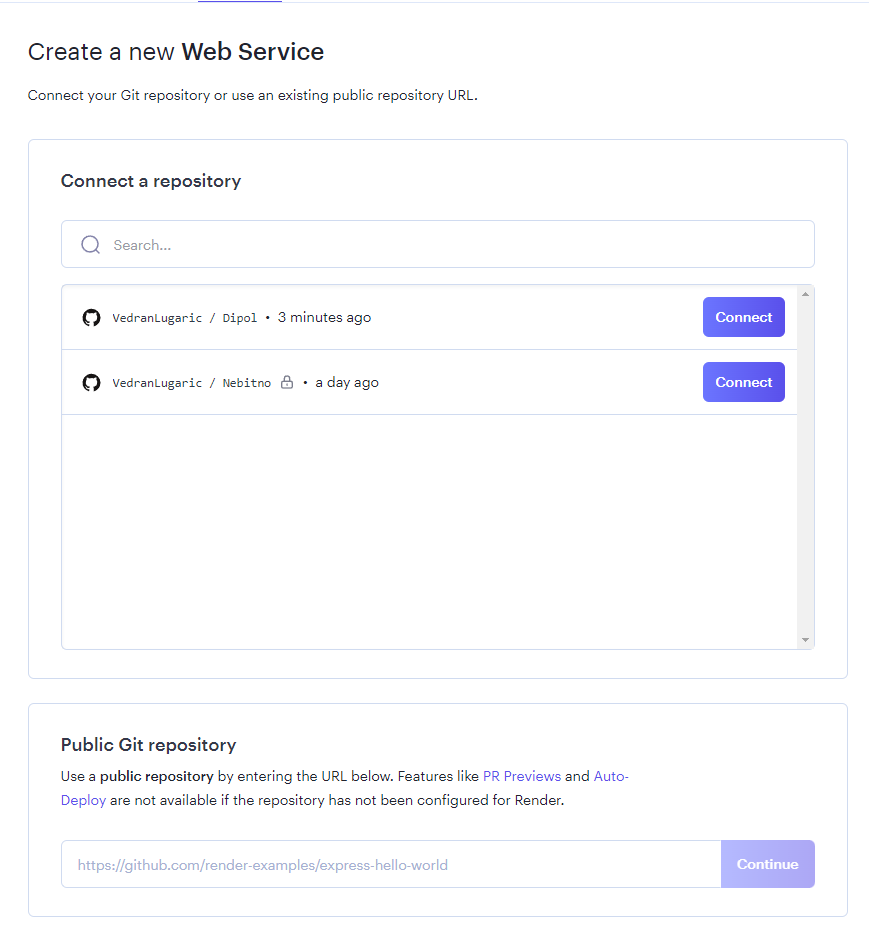
\includegraphics[width=15cm]{slike/back_4.png}
					\label{fig:fer-logo}
				\end{figure}
				\newpage
				\text{}Popunimo potrebna polja kako je prikazano na slici ispod i odabiremo besplatni plan (napomena: progi ključ se mora kopirati u polje desno od polja gdje piše progu ključ).
				
				\begin{figure}[htb]
					\centering
					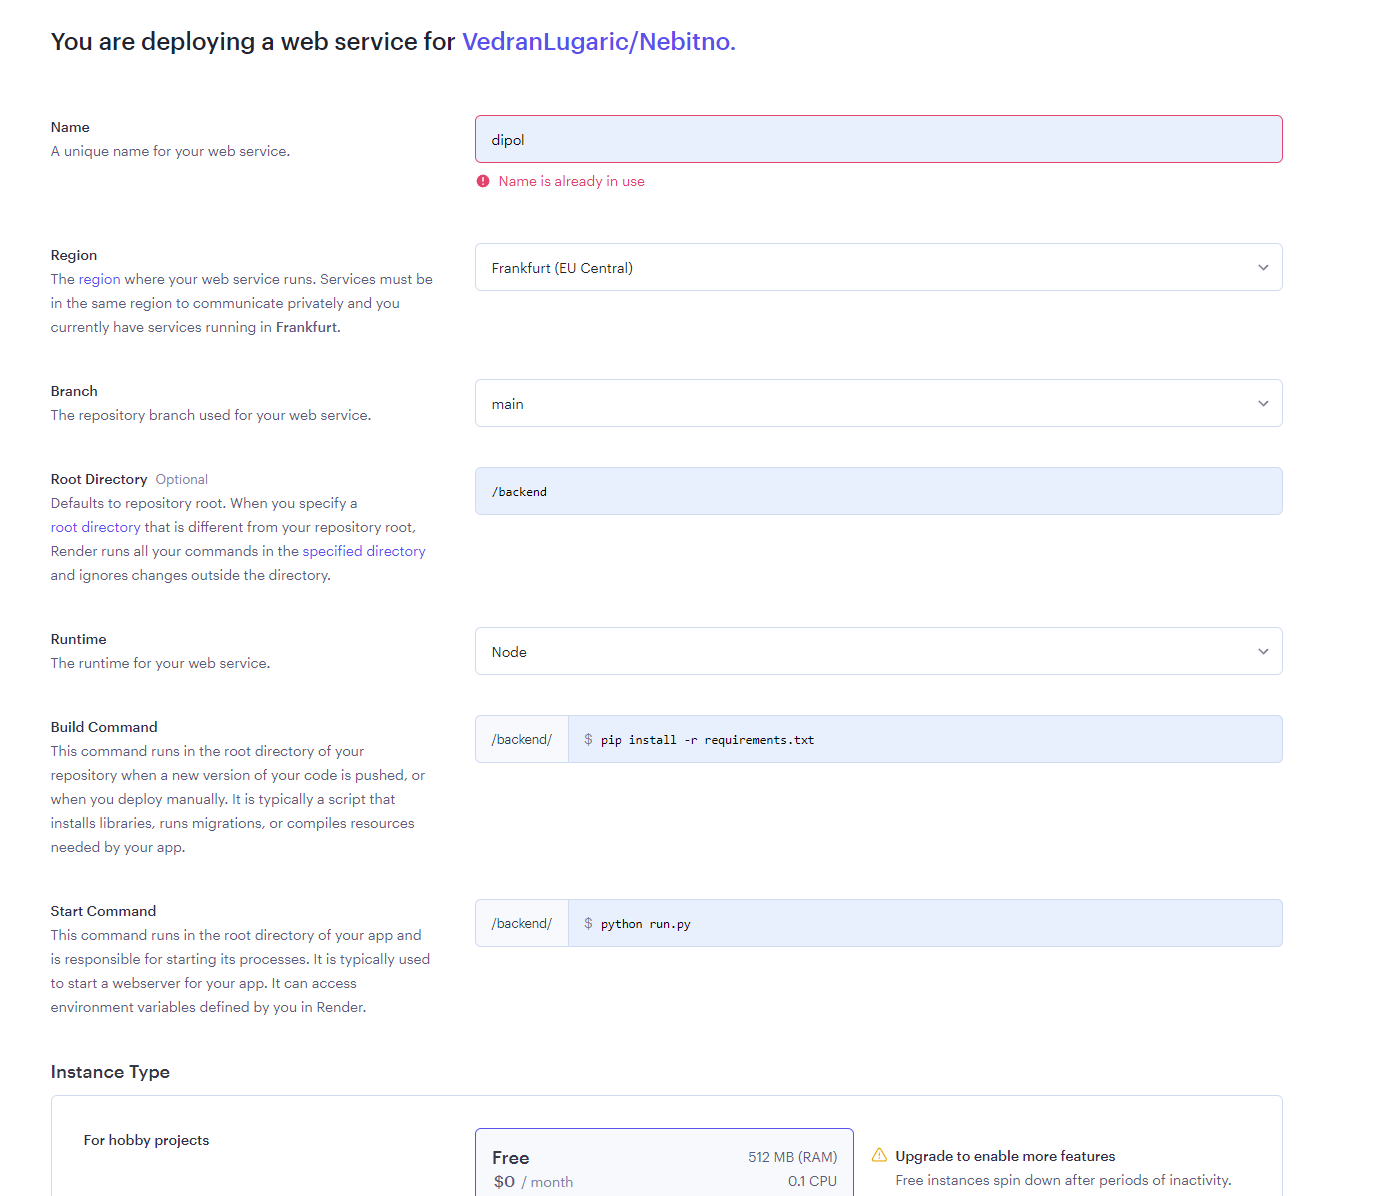
\includegraphics[width=15cm]{slike/back_5.png}
					\label{fig:fer-logo}
				\end{figure}
				\newpage
				\text{}Pritišćemo gumb "Create web service".
				
				\begin{figure}[htb]
					\centering
					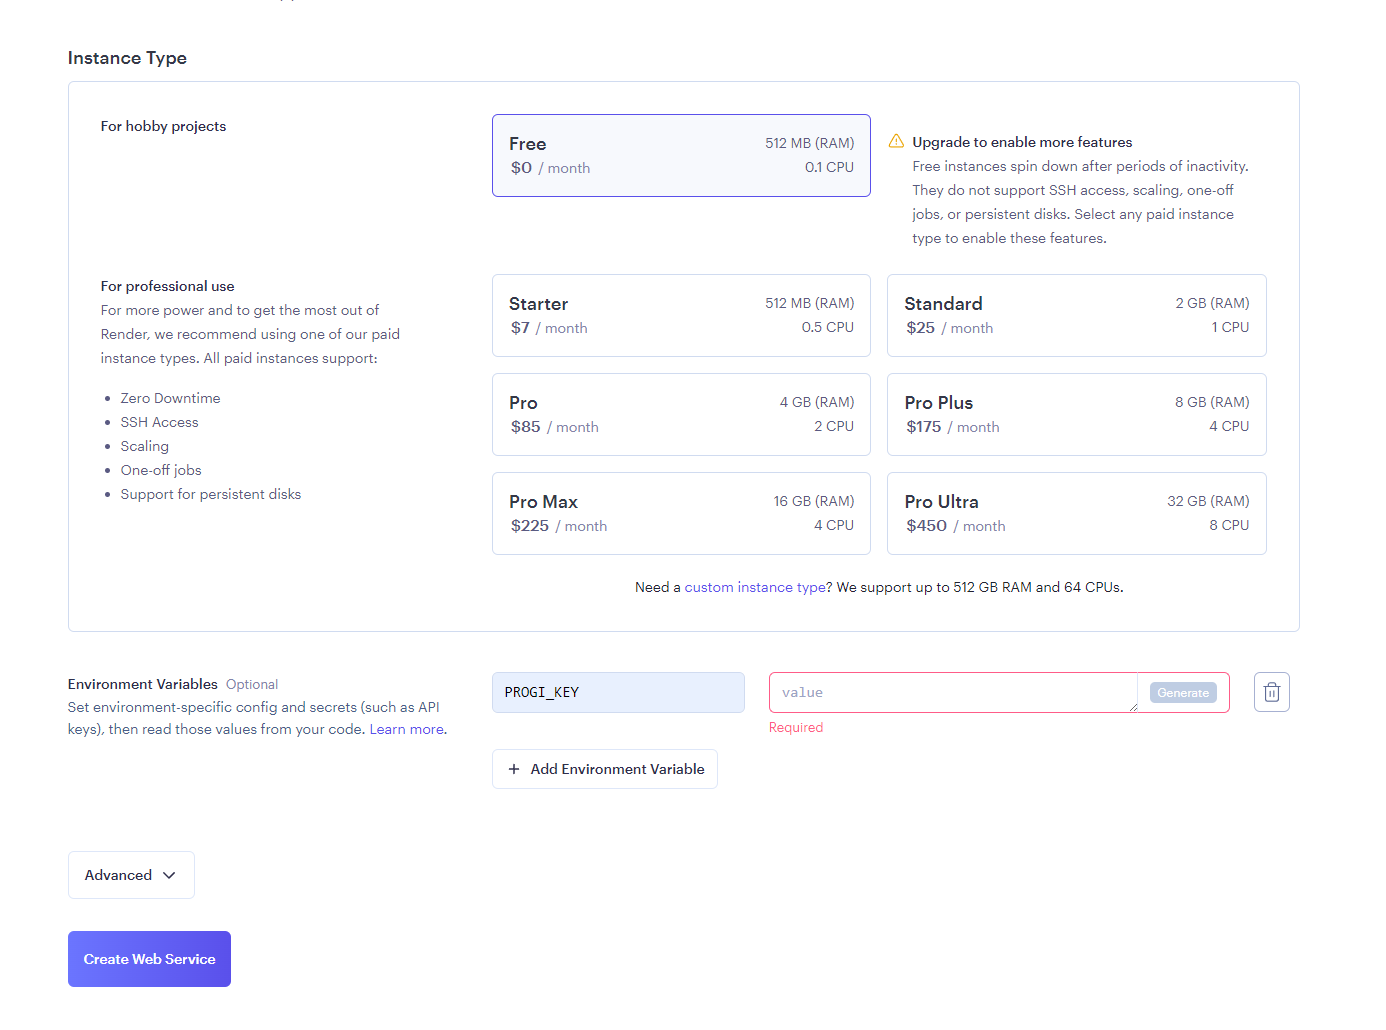
\includegraphics[width=15cm]{slike/back_6.png}
					\label{fig:fer-logo}
				\end{figure}
				\text{}Nakon provedenih svih radnji backend stranice je uspješno pušten u pogon.
			\subsection{Puštanje frontend-a u pogon}
			
				\text{} Frontend pustamo u pogon isto kao i bazu podataka na renderu. Pri pustanju Backenda u pogon na renderu prvo odabiremo gumb "New +" prikazan gore desno na priloženoj slici\\
				
				
				\begin{figure}[htb]
					\centering
					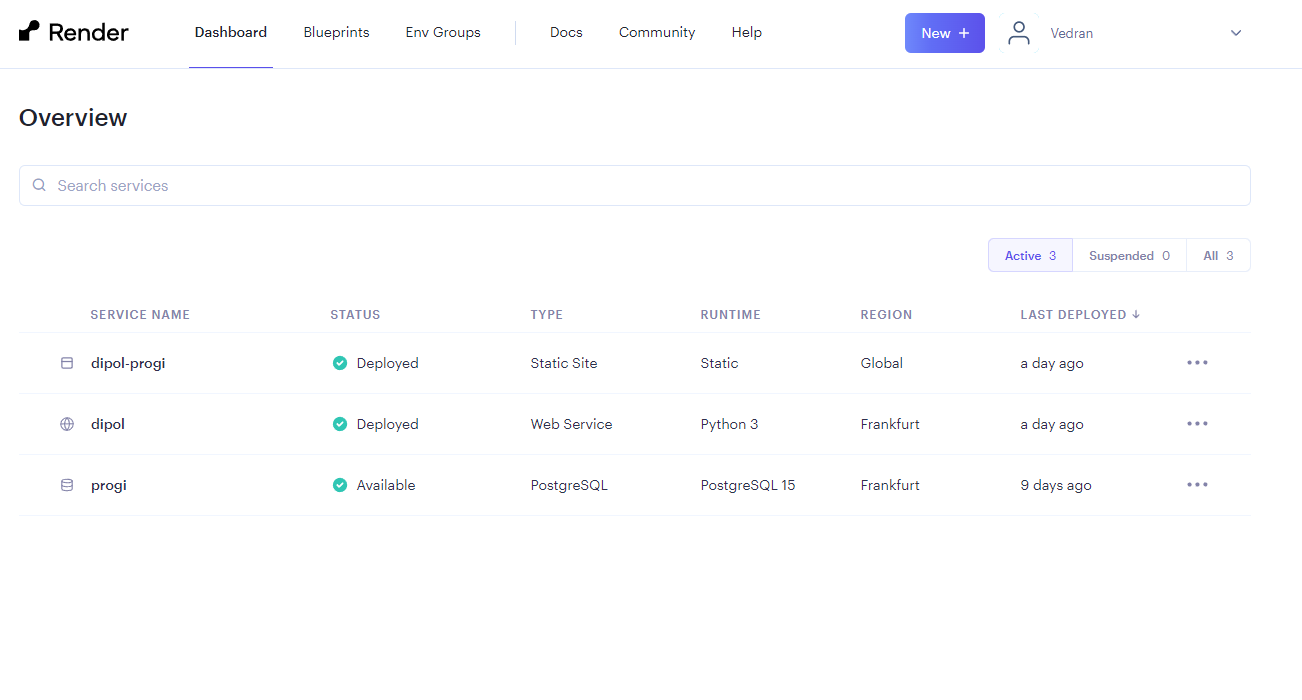
\includegraphics[width=15cm]{slike/back_1.png}
					\label{fig:fer-logo}
				\end{figure}
				\newpage
				\text{}Nakon toga odaibiremo opciju "Static Site".\\
				
				\begin{figure}[htb]
					\centering
					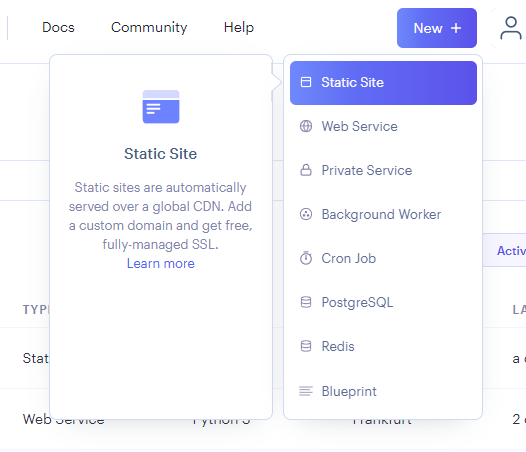
\includegraphics[width=10cm]{slike/front_2.png}
					\label{fig:fer-logo}
				\end{figure}
				\newpage
			
				\text{}Izabiremo server koji želimo pustiti u pogon te na stišćemo na njegov gumb "Connect".
				
				\begin{figure}[htb]
					\centering
					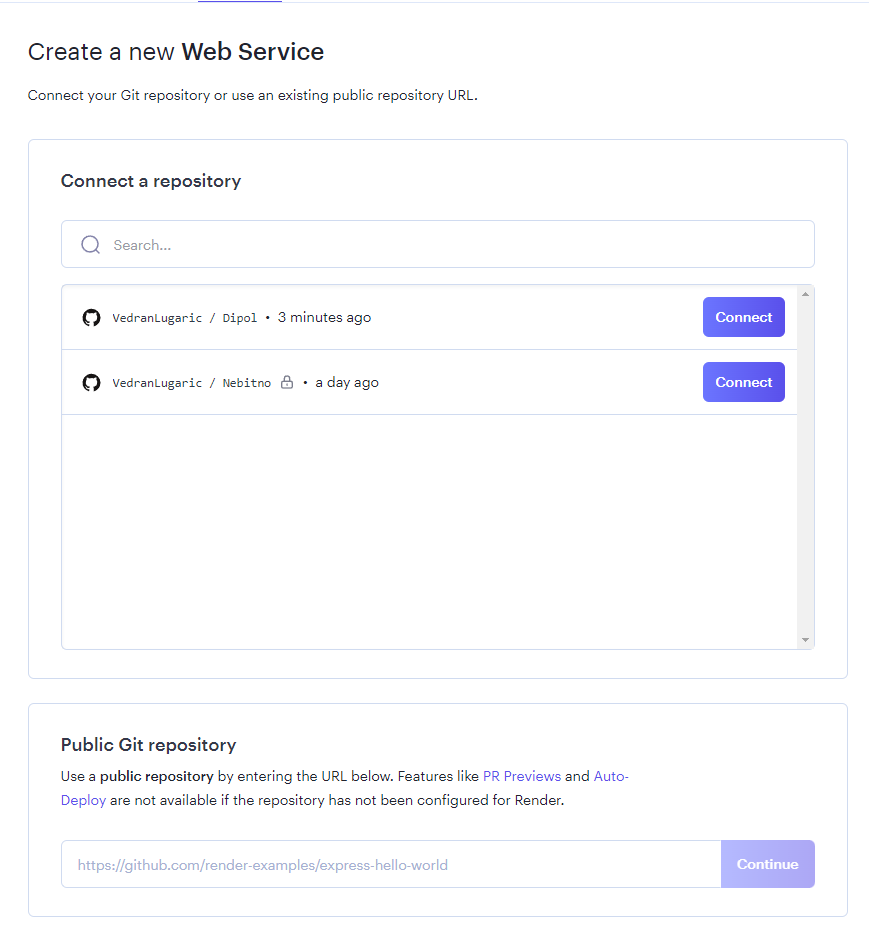
\includegraphics[width=15cm]{slike/back_4.png}
					\label{fig:fer-logo}
				\end{figure}
				\newpage
				\text{}Popunimo potrebna polja kako je prikazano na slici ispod .
				
				\begin{figure}[htb]
					\centering
					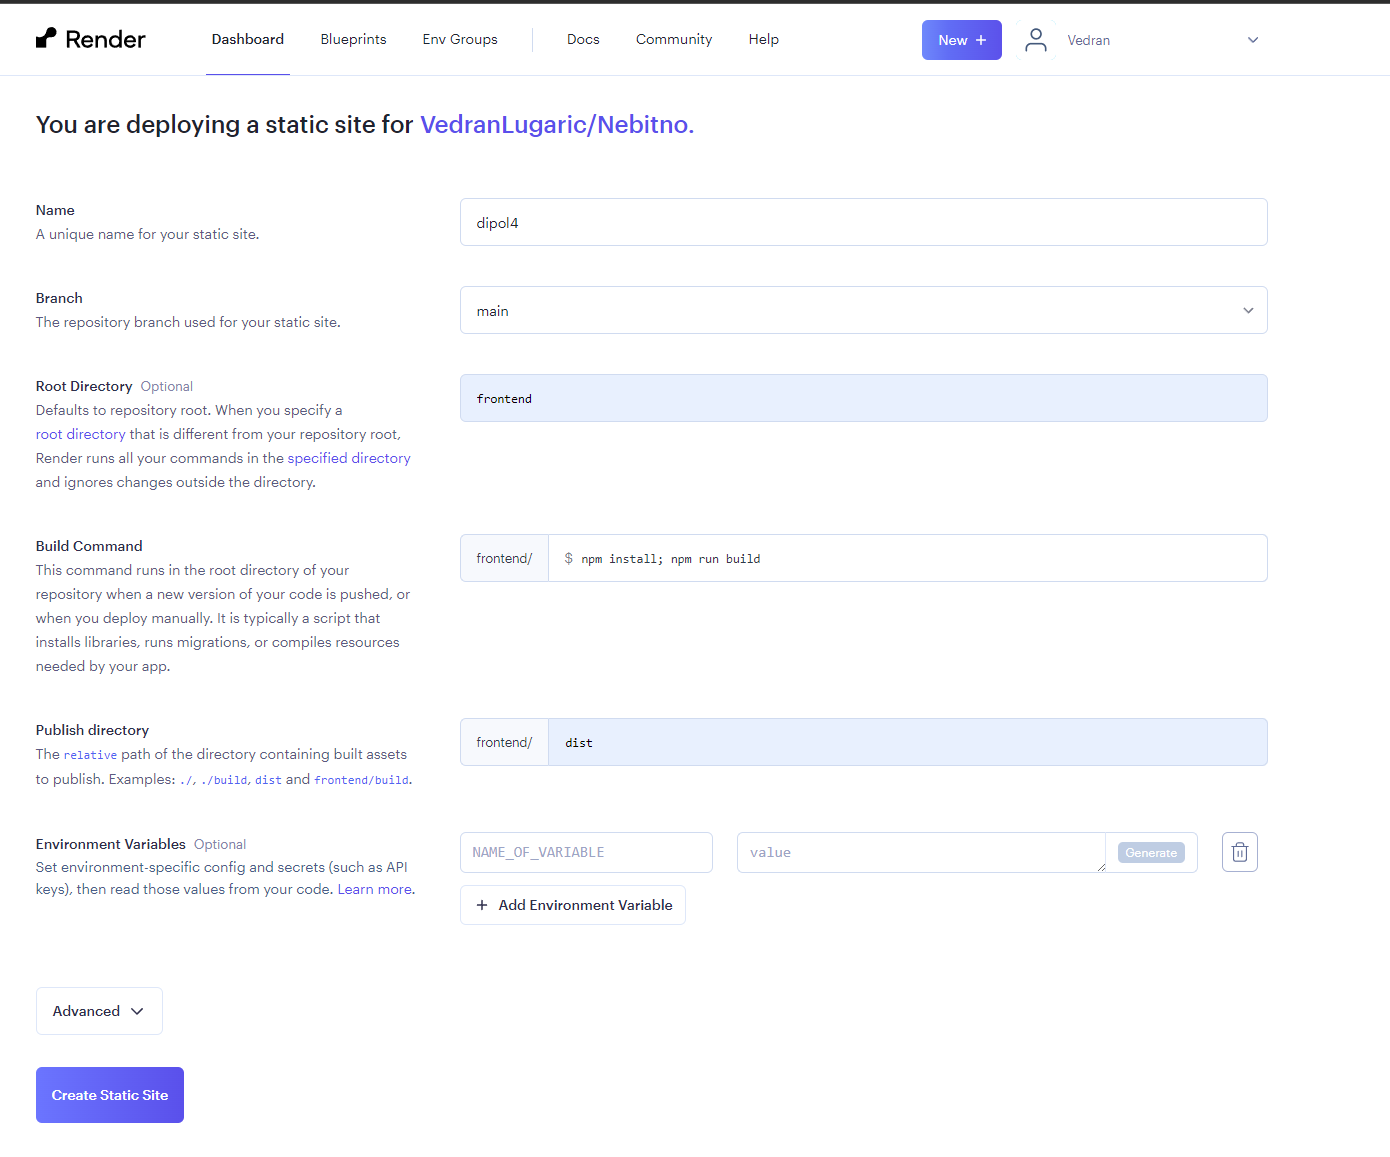
\includegraphics[width=15cm]{slike/front_3.png}
					\label{fig:fer-logo}
				\end{figure}
				
				\text{}Pritišćemo gumb "Create static site".
			
				\text{}Nakon provedenih svih radnji aplikacija je uspješno pušten u pogon.
			
			\eject 